\section{HDR ML Anomaly Challenge (Sea Level Rise)}
{{\footnotesize
\begin{description}[labelwidth=5em, labelsep=1em, leftmargin=*, align=left, itemsep=0.3em, parsep=0em]
  \item[date:] 2025-03-03
  \item[last\_updated:] 2025-03
  \item[expired:] unkown
  \item[valid:] yes
  \item[url:] \href{https://www.codabench.org/competitions/3223/}{https://www.codabench.org/competitions/3223/}
  \item[domain:] Climate Science; Time-series, Image/CV
  \item[focus:] Detecting anomalous sea-level rise and flooding events via time-series and satellite imagery
  \item[keywords:]
    - anomaly detection
    - climate science
    - sea-level rise
    - time-series
    - remote sensing
  \item[task\_types:]
    - Anomaly detection
  \item[ai\_capability\_measured:]
    - Detection of environmental anomalies
  \item[metrics:]
    - ROC‑AUC
    - Precision/Recall
  \item[models:]
    - CNNs, RNNs, Transformers
  \item[ml\_motif:]
    - Time-series, Image/CV
  \item[type:] Dataset
  \item[ml\_task:] Anomaly detection
  \item[notes:] Sponsored by NSF HDR; integrates sensor and satellite data. :contentReference[oaicite:6]\{index=6\}
  \item[contact.name:] HDR A3D3 Team
  \item[contact.email:] unkown
  \item[results.name:] ChatGPT LLM
  \item[results.url:] \href{unkown}{unkown}
  \item[fair.reproducible:] Yes
  \item[fair.benchmark\_ready:] Yes
  \item[ratings.software.rating:] 0
  \item[ratings.software.reason:] TBD
  \item[ratings.specification.rating:] 9.0
  \item[ratings.specification.reason:] Clear anomaly detection objective framed for physical signal discovery (LIGO/Virgo).
  \item[ratings.dataset.rating:] 10.0
  \item[ratings.dataset.reason:] Preprocessed waveform data from dual interferometers, public and well-structured.
  \item[ratings.metrics.rating:] 9.0
  \item[ratings.metrics.reason:] ROC-AUC, Precision/Recall, and confusion-based metrics are standardized.
  \item[ratings.reference\_solution.rating:] 1.0
  \item[ratings.reference\_solution.reason:] No starter model or baseline code linked
  \item[ratings.documentation.rating:] 9.0
  \item[ratings.documentation.reason:] Codabench page, GitHub starter kit, and related papers provide strong guidance.
  \item[id:] hdr\_ml\_anomaly\_challenge\_sea\_level\_rise
  \item[Citations:] \cite{campolongo2025buildingmachinelearningchallenges}
  \item[Ratings:]
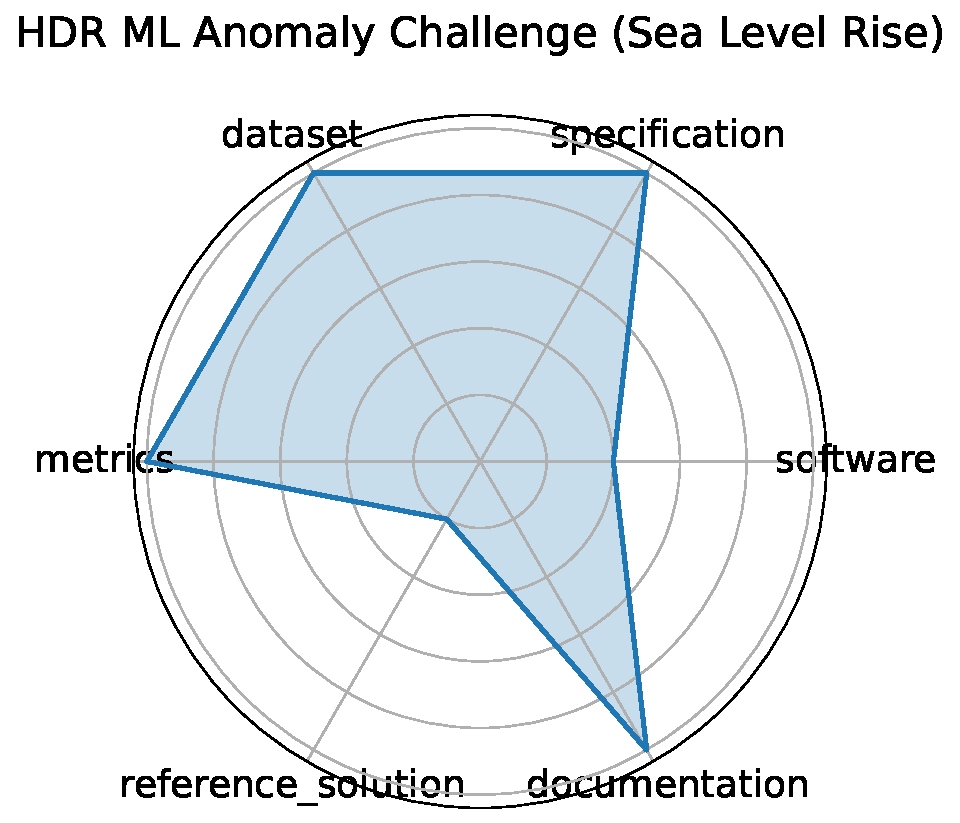
\includegraphics[width=0.2\textwidth]{hdr_ml_anomaly_challenge_sea_level_rise_radar.pdf}
\end{description}
}}
\clearpage